\newcommand{\lscnsource}[1]{
    \scnaddlevel{1}
        \scneq{#1}
    \scnaddlevel{-1}
}

\newcommand{\lscnquote}[2]{
    \scnrelfrom{цитата}{#1}
    \scnaddlevel{1}
        \scneq{\scnfileitem{#2}}
    \scnaddlevel{-1}
}

\begin{SCn}
\begin{small}

\subsection{Предложения к включению в раздел <<Библиотека многократно используемых компонентов OSTIS>>}

\scnheader{Библиотека многократно используемых компонентов OSTIS}\\
...\\
\scnrelfromset{направления развития}{
    уточнение требований к библиотеке многократно используемых компонентов;
    уточнение технологии разработки многократно используемых компонентов
}
\scnrelfrom{технология}{компонентое программное обеспечение}

\scnheader{компонентное программное обеспечение}
\scndefinition{...компонентное программное обеспечение является конструкцией из компонентов, часть из которых могут быть серийными компонентами, а другие — изготовленными на заказ.}
\scnaddlevel{1}
    \scneq{Quote.Phister.C.ComponentSoftware-1997art.p4}
\scnaddlevel{-1} 
\scnsubset{COTS-программное обеспечение}
% It is very difficult to guess how the components behave under different conditions and environments as mostly COTS software comes up as a black box with limited access.
\scnrelfromset{проблемы текущего состояния}{
    \scnfileitem{Сложно предугадать, каким оьразом поведут себя компоненты в различных условиях и окружениях, так как обычно COTS-программное обеспечение поставляется в виде чёрного ящика с ограниченным доступом.}
    \scnaddlevel{1}
        \scneq{Quote1.Khan.A.PerspecStudyISFCBD-2015art.p11}
    \scnaddlevel{-1};
    % It is also difficult to map user requirement to the component based architecture and generally there is a need for a process which fully customized the component as per the customer requirement. 
    \scnfileitem{Также сложно удовлетворить требования пользователя при использовании компонентно-ориентированной архитектуры, обычно необходим процесс подробной настройки компонента.}
    \scnaddlevel{1}
        \scneq{Quote2.Khan.A.PerspecStudyISFCBD-2015art.p11}
    \scnaddlevel{-1};
    % In order to developed application from components or tailor components to a new situation, efforts are required to build wrappers and the glue between components, since most of the COTS software lacks in plug and play technique and developer has to build wrappers for component integration. Further, wrappers need to be maintained as the system evolves.
    \scnfileitem{Для разработки приложения из компонинтов или улучшения поведения компонентов, необходимо создавать "обёртки" и "склеивать" компоненты, полскольку большая часть COTS-программного обеспечения лишена технологии plug and play и разработчику приходить вручную создавать "обёртки" для интеграции компонентов. Мало того, "обёртки" необходимо поддерживать, пока поддерживается сама система.}
    \scnaddlevel{1}
        \scneq{Quote.Khan.A.PerspecStudyISFCBD-2015art.p11-12}
    \scnaddlevel{-1};
    % Components are packaged and delivered in many different forms (example: function libraries, off-the shelf applications and frameworks). 
    \scnfileitem{Компоненты упаковываются и доставляются во многих различных формах (например, библиотеки функций, COTS-приложения, фреймворки).}
    \scnaddlevel{1}
        \scneq{Quote1.Khan.A.PerspecStudyISFCBD-2015art.p12}
    \scnaddlevel{-1};
    % Most component integration processes suffer from inflexibility by a lack of component evaluation schemes. This problem is often compounded by a lack of interoperability standards between component frameworks and adequate vendor support.
    \scnfileitem{Зачастую процесс интеграции компонентов страдает от негибкости и нехватки схем оценки компонентов. Это проблема зачастую сопровождается отстутствием стандартов интероперабельности между компонентами и адекватной поддержки от производителя.}
    \scnaddlevel{1}
        \scneq{Quote2.Khan.A.PerspecStudyISFCBD-2015art.p12}
    \scnaddlevel{-1}
}
\scnrelfromset{требования}{
    \scnfileitem{Фундаментальное требование к компонентному ПО состоит в том, чтобы компоненты могли разрабатываться и продаваться независимо друг от друга, и, таким образом, могли комбинироваться потребителем.}
    \scnaddlevel{1}
        \scneq{Quote2.Phister.C.ComponentSoftware-1997art.p3}
    \scnaddlevel{-1};
    \scnfileitem{
        \begin{scnitemize}
            \item стандарт, который допускает динамическую загрузку компонентов (динамически загружаемые библиотеки, соглашения вызовов)
            \item стандартный программный интерфейс
            \item механизм защиты, который предотвращает нелегальные изменения состояний одних компонентов другими
            \item способ разделения данных между компонентами без их копирования взад-вперед и без явных преобразований в линейные потоки байт
        \end{scnitemize}
    }
    \scnaddlevel{1}
        \scneq{Quote2.Phister.C.ComponentSoftware-1997art.p15}
    \scnaddlevel{-1}
}
\scnrelfromset{достоинства}{
    \scnfileitem{При разбиении сложной проблемы на более простые, которые могут быть решены независимо друг от друга, проблема становится более управляемой.}
    \scnaddlevel{1}
        \scneq{Quote.Phister.C.ComponentSoftware-1997art.p4-5}
    \scnaddlevel{-1};
    \scnfileitem{Компоненты могут разрабатываться параллельно, если заранее ясно определено, что каждый компонент должен предоставлять, так что программист может немедленно использовать интерфейс компонента, который разрабатывается другим сотрудником — даже если его реализация еще не существует.}
    \scnaddlevel{1}
        \scneq{Quote1.Phister.C.ComponentSoftware-1997art.p5}
    \scnaddlevel{-1};
    \scnfileitem{В программном проекте может случиться так, что кто-то вспомнит, что какая-либо часть текущей задачи уже была решена в предыдущем проекте. Если это частичное решение было оформлено как независимый компонент, оно может быть повторно использовано в новом проекте. При этом произойдет экономия времени и средств.}
    \scnaddlevel{1}
        \scneq{Quote2.Phister.C.ComponentSoftware-1997art.p5}
    \scnaddlevel{-1};
    \scnfileitem{Они [покупатели] могут сэкономить время за счет покупки компонентов на рынке, и тем самым снижают вероятность того, что программные решения уже устареют к моменту своей готовности. Компонентное ПО позволяет добавлять со временем новую функциональность, присоединяя новые компоненты к уже существующим решениям. Таким образов, решение может расширяться, чтобы соответствовать новым нуждам.}
    \scnaddlevel{1}
        \scneq{Quote3.Phister.C.ComponentSoftware-1997art.p5}
    \scnaddlevel{-1}
}
\scnrelfromset{недостатки}{
    \scnfileitem{Компонентная реализация — все еще трудная инженерная проблема. Проектирование интерфейсов компонент даже еще более вызывающе. Это требует хорошо образованных и опытных инженеров. Разработка действительно многоразовых высококачественных компонентов не может быть совершена «одним выстрелом»; она требует итеративного долговременного совершенствования, и потому является дорогостоящей.}
    \scnaddlevel{1}
        \scneq{Quote.Phister.C.ComponentSoftware-1997art.p7}
    \scnaddlevel{-1}
}
\scnrelbothlist{следует отличать}{объектно-ориентированное программное обеспечение;модульное программное обеспечение}
\scnaddlevel{1}
    \scnrelfromlist{пояснение}{
        \scnfileitem{Программный компонент -- то, что непосредственно разворачивается -- как изолируемая часть системы -- в компонентно-ориентированном подходе. Вопреки частым утверждениям, объекты почти никогда не продаются, не покупаются и не разворачиваются.}
        \scnaddlevel{1}
            \scneq{Quote.Szyperski.C.CompSoftBOOP-2002book.p10}
        \scnaddlevel{-1};
        \scnfileitem{...при разработке компонента также может быть использована совсем иная технология, такая как чистые функции или язык ассемблера, которые не имеют ничего общего с объектно-ориентированностью изнутри.}
        \scnaddlevel{1}
            \scneq{Quote1.Szyperski.C.CompSoftBOOP-2002book.p11}
        \scnaddlevel{-1};
        \scnfileitem{Определение [объекта] не включает в себя независимости или компонуемости.}
        \scnaddlevel{1}
            \scneq{Quote2.Szyperski.C.CompSoftBOOP-2002book.p11}
        \scnaddlevel{-1}
    }
\scnaddlevel{-1}
\scnhaselement{многократно используемый компонент}
\scnhaselement{объектная модель}

\scnheader{COTS-программное обеспечение}
\scnexplanation{
    Commercially available off-the-shelf (COTS) означает любой предмет продажи (включая материалы для сборки), которые:
    \begin{scnitemize}
        \item Являются коммерческим продуктом
        \item Продаются в значительных количествах на коммерческом рынке
        \item Предлагаются Правительству [заказчику] контрактом любого уровня, без модификаций, в той же форме, в которой он продаётся на коммерческом рынке
    \end{scnitemize}
}
\scnaddlevel{1}
    \scneq{Quote.USGenServAdm.2.101.Definitions-reg}
\scnaddlevel{-1}



\scnheader{объектная модель}
\scndefinition{Объектная модель определяет необходимые правила совместимости компонентов на уровне двоичного [машинного] кода, так что компоненты могут взаимодействовать на конкретной машине, даже если они разрабатывались независимо.}
\scnaddlevel{1}
    \scneq{Quote.Phister.C.ComponentSoftware-1997art.p18}
\scnaddlevel{-1}
\scnhaselement{язык определения интерфейсов}
\scnhaselement{репозиторий интерфейсов}
\scnhaselement{формат динамически компонуемых библиотек}
\scnhaselement{репозиторий реализации}
\scnhaselement{компонующий загрузчик}
\scnhaselement{механизм для проверки версий загружаемого кода}
\scnhaselement{механизм для создания экземпляров загруженного компонента}
\scnhaselement{соглашения по вызову методов компонента}
\scnhaselement{механизм для навигации между полиморфными типами компонента}
\scnhaselement{формат сообщений}
\scnhaselement{механизм уничтожения объектов}
\scnaddlevel{1}
    \scneq{sc-агент обнаружения и удаления информационного мусора}
\scnaddlevel{-1}

\scnheader{язык определения интерфейсов}
\scnidtf{IDL}
\scnidtf{interface description language}
\scnexplanation{Компонент может пользоваться услугами другого компонента. Для этого разработчику надо всего лишь знать интерфейс используемого компонента. Возможно, для этого интерфейса пока еще даже нет реальной реализации. Интерфейс должен быть некоторым образом описан. Текстовое описание интерфейса записывается на языке описания интерфейса (IDL, interface description language). В идеале, он должен быть подмножеством того языка, который использует разработчик. Однако в целом объектная модель независима от языка, и конечно же, IDL может быть подмножеством только лишь очень похожих языков программирования.}
\scnaddlevel{1}
    \scneq{Quote.Phister.C.ComponentSoftware-1997art.p18-19}
\scnaddlevel{-1}

\scnheader{репозиторий интерфейсов}
\scnexplanation{IDL-описание предоставляет разработчику информацию об интерфейсе объекта. Если возможно, компилятор должен использовать такую информацию для проверки того, корректно ли используется интерфейс. В этих целях часто существует двоичный формат для описание интерфейсов, в дополнение к текстовому IDL-формату. Доступный набор таких двоичных описаний называется репозиторием интерфейсов. Он может состоять просто из набора так называемых символьных файлов, или он может храниться в базе данных какого-либо рода.}
\scnaddlevel{1}
    \scneq{Quote1.Phister.C.ComponentSoftware-1997art.p19}
\scnaddlevel{-1}

\scnheader{формат динамически компонуемых библиотек}
\scnexplanation{Когда компонент компилируется, компилятор должен создать файл, который содержит сгенерированный код. Формат такого файла должен подходить для загрузки во время выполнения, то есть, он должен быть динамически загружаемой библиотекой.}
\scnaddlevel{1}
    \scneq{Quote2.Phister.C.ComponentSoftware-1997art.p19}
\scnaddlevel{-1}

\scnheader{репозиторий реализации}
\scnexplanation{Во время выполнения, когда компоненту первый раз потребовались услуги другого компонента, тот компонент загружается. Загрузчик сначала находит кодовый файл для компонента. Расположение кодового файла может быть очевидным, например, имя компонента может напрямую определять путь к его кодовому файлу в файловой системе. Другой вариант - текущее положение кодового файла может запрашиваться из конфигурационной базы данных. Косвенный подход более гибок, но более требователен в плане системного администрирования. Набор кодовых файлов или соответствующая база данных называются репозиторием реализации.}
\scnaddlevel{1}
    \scneq{Quote3.Phister.C.ComponentSoftware-1997art.p19}
\scnaddlevel{-1}

\scnheader{механизм для проверки версий загружаемого кода}
\scnexplanation{Когда загрузчик успешно нашел компонент и загрузил его код в память, он может проверить, действительно ли загруженный код реализует запрошенный интерфейс, и совместимы ли версии загруженного компонента и его клиента. Такая проверка — насущная необходимость, поскольку нельзя допустить, чтобы кофликт версий привел некоторое время спустя к краху, и при этом пользователь мог бы только догадываться о причине проблемы. Некоторые объектные модели не предоставляют адекватного механизма контроля версий и перекладывают бремя проверки соответствия частично и полностью на клиентский компонент.}
\scnaddlevel{1}
    \scneq{Quote4.Phister.C.ComponentSoftware-1997art.p19}
\scnaddlevel{-1}

\scnheader{механизм для создания экземпляров загруженного компонента}
\scnexplanation{Как только код компонента загружен и проверен, могут быть созданы экземпляры его классов. Для этих целей объектная модель должна обладать механизмом размещения объектов. Некоторые объектные модели предлагают косвенный подход к размещению, чтобы дать дополнительную гибкость. В частности, объект может создаваться другим объектом, так называемой фабрикой. Объект-фабрика может сам решать, как размещать и как инициализировать объекты.}
\scnaddlevel{1}
    \scneq{Quote5.Phister.C.ComponentSoftware-1997art.p19}
\scnaddlevel{-1}

\scnheader{соглашения по вызову методов компонента}
\scnexplanation{После того, как объект был создан и стал доступен для других, можно вызывать его методы. Вызов метода — это вызов процедуры, который выполняется не напрямую, а через объект, так что различные объекты могут приводить к вызову различного кода. Обычно объект содержит указатель на таблицу указателей на процедуры. Каждый элемент этой таблицы соответствует одному методу объекта. Поэтому вызов метода - всего лишь непрямой вызов процедуры через таблицу методов объекта. Обычно для этих вызовов используются соглашения вызовов базовой операционной системы.}
\scnaddlevel{1}
    \scneq{Quote6.Phister.C.ComponentSoftware-1997art.p19}
\scnaddlevel{-1}

\scnheader{механизм для навигации между полиморфными типами компонента}
\scnexplanation{Полиморфизм — одно из главных качеств любой объектно-ориентированной или компонентно-ориентированной системы. Некотрый интерфейс, поддерживаемый объектом, может быть известен во время компиляции. Он называется его статическим типом. Но объект может приобретать дополнительные возможности, то есть, расширять свой интерфейс, во время выполнения. В зависимости от динамического типа объекта эти возможности могут отличаться. Это называется полиморфизмом («много форм»). Объектная модель должна обеспечить средства, с помощью которых можно получить доступ к таким дополнительным возможностям, если и только если они доступны. Объектно-ориентированный язык программирования в этих целях задает языковые конструкции, такие как расширение типа (также извествное как субтипизация или наследование интерфейса), проверки типа или охрана типа (то есть, безопасные преобразования между типами). Объектная модель может предоставлять похожую функциональность. Без полифморфизма система не может быть расширяемой.}
\scnaddlevel{1}
    \scneq{Quote1.Phister.C.ComponentSoftware-1997art.p20}
\scnaddlevel{-1}

\scnheader{механизм уничтожения объектов}
\scnexplanation{Если объект больше не используется, то есть, на него больше нет внешних ссылок, он должен быть уничтожен, чтобы освободилась занимаемая им память. В компонентных системах на объект, который компонент предоставляет вовне, ссылаются какие-либо другие объекты, о которых сам объект ничего не знает. Поэтому должны существовать правила, которые указывают, кто и когда должен уничтожить данный объект. Например, это может сделать другой объект, у которого осталась последняя ссылка на данный. Для определения того момента, когда ссылка на объект стала последней, необходим механизм трассировки ссылок, например, счетчик ссылок в каждом объекте, который подсчитывает количество текущих ссылок на него. Когда количество становится равным нулю, память объекта может быть освобождена. Для того, чтобы такие правила работали, критически важно их правильное использование всеми компонентами. В замкнутых приложениях неправильная работа с памятью является самым главным источником ошибок; но вы, по крайней мере, знаете, кто виноват в произошедшем сбое. В открытых компонентных системах один неправильно работающий компонент может привести к краху всю систему, при этом сложно определить виновного производителя. Поэтому управление памятью в компонентной программной среде является принципиально более важным вопросом, чем в монолитном ПО. В идеале правила и механизмы, вводимые объектной моделью, должны быть достаточно простыми, полными и ясными, чтобы их можно было автоматизировать, то есть, освободить разработчика от ручной работы, предоставив автоматический сборщик мусора. Автоматический сборщик мусора в открытых системах - это не роскошь, а необходимость.}
\scnaddlevel{1}
    \scneq{Quote2.Phister.C.ComponentSoftware-1997art.p20}
\scnaddlevel{-1}

\scnheader{формат сообщений}
\scnexplanation{Объектная модель, которая поддерживает распределенные объекты, должна определять формат сообщений, который описывает потоки байт, порождаемые удаленным вызовом методов. Того, кто вызывает метод, называют клиентом, того, чей метод вызывают, — сервером. По самому общему сценарию серверный объект и клиент выполняются на разных машинах. С точки зрения разработчика клиент может напрямую вызывать методы серверного объекта. В реальности клиент взаимодействует всего лишь с прокси-объектом, который является локальным представителем настоящего объекта, работающего на удаленной серверной машине. В большинстве реализаций прокси-объект, также как и его аналог на стороне сервера, могут генерироваться автоматически из интерфейса объекта.}
\scnaddlevel{1}
    \scneq{Quote3.Phister.C.ComponentSoftware-1997art.p20}
\scnaddlevel{-1}

\scnheader{многократно используемый компонент}
\scndefinition{Компонент — это элемент конструкции с определенным, зафиксированным в спецификации, интерфейсом и явными зависимостями от контекста. Компоненты могут распространяться независимо друг от друга и компоноваться третьей стороной.}
\scnaddlevel{1}
    \scneq{Quote.Phister.C.ComponentSoftware-1997art.p3}
\scnaddlevel{-1}
\scnrelfromset{требования}{
    независимость многократно используемого компонента;
    компонуемость многократно используемого компонента;
    скрытое внутреннее состояние многократно используемого компонента;
    уникальность многкратно используемого компонента
}
\scnrelfromset{декомпозиция}{
    интерфейс многократно используемого компонента;
    реализация многократно используемого компонента
}

\scnheader{независимость многократно используемного компонента}
\scnexplanation{Для того, чтобы компонент можно было развернуть независимо, он должен быть отделён от своего окружения и других компонентов.}
\scnaddlevel{1}
    \scneq{Quote1.Szyperski.C.CompSoftBOOP-2002book.p36}
\scnaddlevel{-1}

\scnheader{компонуемость многократно используемого компонента}
\scnexplanation{...он [компонент] должен поставляться с чёткой спецификацией того, что он требует и предоставляет. Другими словами, компонент должен скрывать свою имплементацию и взаимодействовать с окружением при помощи чётко определённых интерфейсов.}
\scnaddlevel{1}
    \scneq{Quote2.Szyperski.C.CompSoftBOOP-2002book.p36}
\scnaddlevel{-1}

\scnheader{скрытое внутреннее состояние многократно используемного компонента}
\scnexplanation{...компонент не должен иметь наблюдаемого (извне) состояния.}
\scnaddlevel{1}
    \scneq{Quote3.Szyperski.C.CompSoftBOOP-2002book.p36}
\scnaddlevel{-1}

\scnheader{уникальность многократно используемого компонента}
\scnexplanation{...не имеет смысла иметь несколько копий [компонента] в одной и той же операционной системе, поскольку они в любом случае будут фактически неотличимы. Другими словами, в любом процессе (или ином контексте), не должно быть более одной копии конкретного компонента.}
\scnaddlevel{1}
    \scneq{Quote4.Szyperski.C.CompSoftBOOP-2002book.p36}
\scnaddlevel{-1}

\scnheader{интерфейс многократно используемого компонента}
\scndefinition{Интерфейс определяет стандарт, которому производители компонентов обязаны следовать и которого пользователи вправе ожидать.}
\scnaddlevel{1}
    \scneq{Quote.Phister.C.ComponentSoftware-1997art.p15}
\scnaddlevel{-1}
\scnexplanation{...каждому компоненту нужно взаимодействовать с другими компонентами исключительно через их интерфейсы; это разновидность контракта, иначе говоря, закон для программиста.}
\scnaddlevel{1}
    \scneq{Quote1.Phister.C.ComponentSoftware-1997art.p17}
\scnaddlevel{-1}
\scnrelboth{следует разделять}{реализация многократно используемого компонента}
\scnrelfromset{требования}{
    ясность интерфейса многократно используемого компонента;
    существенность интерфейса многократно используемого компонента
}

\scnheader{ясность интерфейса многократно используемного компонента}
\scnexplanation{В то время как синтаксис интерфейса может быть задан очень легко, ясная семантика трудноуловима. Обычно имеется простой неформальный текст, который описывает, что из себя представляет некоторый интерфейс. Формальные и полуформальные методы специфицирования могут помочь сделать интерфейсы менее противоречивыми.}
\scnaddlevel{1}
    \scneq{Quote.Phister.C.ComponentSoftware-1997art.p16}
\scnaddlevel{-1}

\scnheader{существенность интерфейса многократно используемого компонента}
\scnexplanation{Интерфейс, который задает слишком много несущественных деталей, заставит программистов использовать их и допускать их истинность. Становится невозможным изменить эти детали позже, даже если это действительно потребуется.}
\scnaddlevel{1}
    \scneq{Quote2.Phister.C.ComponentSoftware-1997art.p17}
\scnaddlevel{-1}

\pagebreak

\subsection{Предложения к включению в раздел <<Предметная область и онтология интерфейсов ostis-систем>>}

\scnheader{пользовательский интерфейс}
\scnsuperset{графический пользовтельский интерфейс}
\scnaddlevel{1}
    \scnsuperset{WIMP-интерфейс}
    \scnaddlevel{1}
        \scnsuperset{IUI-интерфейс}
            \scnaddlevel{1}
                \scnsuperset{мультимодальный интерфейс}
                \scnsuperset{естественно-языковой интерфейс}
                \scnaddlevel{1}
                    \scnsuperset{речевой интерфейс}
                \scnaddlevel{-1}
                \scnsuperset{мимический интерфейс}
                \scnsuperset{жестовый интерфейс}
            \scnaddlevel{-1}
    \scnaddlevel{-1}
\scnaddlevel{-1}

\scnheader{IUI-интерфейс}
\scnidtf{intelligent user interface}
\scnidtf{IUI}
\scnexplanation{Интеллектуальные пользовательские интерфейсы (IUI) — это человеко-машинные интерфейсы, целью которых является повышение эффективности, результативности и естественности взаимодействия человека и машины путем представления, рассуждений и действий на основе моделей пользователя, предметной области, задачи, дискурса и медиа (например, , графика, естественный язык, жест). Как следствие, эта междисциплинарная область опирается на исследования и лежит на пересечении взаимодействия человека с компьютером, эргономики, когнитивной науки и искусственного интеллекта и его подобластей (например, компьютерное зрение, обработка речи и языка, представление знаний и рассуждения, машинное обучение/обнаружение знаний, планирование и агентное моделирование, пользовательское и дискурсивное моделирование).}
\lscnsource{Quote1.Maybury.M.IntellUserInterfIntro-1998art.p2}
\scnrelfrom{цели}{\scnfileitem{
    \begin{scnitemize}
        \item \textbf{Создание персонализированных систем}\\
        Не существует двух людей с одинаковыми привычками, предпочтениями, методами работы и окружением. Интеллектуальный интерфейс, который учитывает все эти различия может создать персонализованный метод взаимодействия. Интерфейс знает пользователя и может использовать это знание для общения с пользователем.
        \item \textbf{Перегрузка информацией и проблемы фильтрации}\\
        Найти правильную информацию на компьютере или в сети может быть сложнее, чем найти нитку в стоге сена. Интеллектуальные интерфейсы могут снизить перегрузку информацией, которая возникает при поиске в больших базах данных или сложных системах. При помощи фильтрации неважной информации интерфейс может снизить когнитивную нагрузку на пользователя. К тому же, IUI может предложить новые и полезные источники, о которых пользователь ранее не знал.
        \item \textbf{Помощь в пользовании новым и сложным ПО}\\
        Работа с компьютерными системами может быть сложна, особенно, если это первый опыт пользователя в работе с конкретным ПО. Пока пользователь пытается разобраться с новой программой, новые версии ПО и прочие обновления могут добавить новый функционал. Многие пользователи не успевают за всеми этими обновлениями. Интеллектуальные вспомогательные системы могут обнаруживать и исправлять недопонимания пользователя, объяснять новые концепции, снабжать пользователя информацией для упрощения работы.
        \item \textbf{Делегирование задач от пользователя}\\
        IUI, во время действия пользователя, может понимать и узнавать намерение пользователя и даже забрать себе часть работы пользователя, позволяя ему сфокусироваться на более важных задачах.
        \item \textbf{Прочие формы взаимодействия}\\
        На данный момент, наиболее распространенные средства взаимодействия -- клавиатура и мышь. IUI также рассматривает иные способы взаимодействия компьютера и человека (например, речь или жесты). Альтернативные формы взаимодействия могут помочь людям с ограниченными возможностями проще пользоваться компьютером.
    \end{scnitemize}
}
\lscnsource{Quote1.Ehlert.P.IntellUserInterfIAS-2003art.p2}}

\scnrelfrom{требования}{\scnfileitem{
\begin{scnitemize}
    \item Адаптивный пользовательский интерфейс должен разрабатываться параллельно с приложением. Это необходимо, так как разработчику постоянно приходится сосредотачиваться на частях системы, которые необходимо адаптировать.
    \item Не мешайте взаимодействию пользователя. Пользователь всегда должен иметь возможность игнорировать упреждающие действия IUI. Предлагайте, а не действуйте.
    \item Работайте в режиме реального времени. Большая часть преимуществ IUI заключается в том, что он действует, пока пользователь занят работой с системой.
    \item Воспользуйтесь временем, который пользователь тратит на раздумия. Когда пользователь думает о том, что вводить дальше, IUI может использовать доступное время для своих целей, таким образом он не рискует замедлить взаимодействие пользователя с системой.
    \item Следите за тем, что делает пользователь. Воспользуйтесь преимуществом «бесплатной» информации, скрытой в действиях пользователя.
    \item Позвольте пользователю выбирать свой личный стиль взаимодействия. Разным пользователям нравятся разные стили интерфейса, и некоторые методы могут отвлекать или сбивать с толку некоторых пользователей.
\end{scnitemize}
}\lscnsource{Quote1.Ehlert.P.IntellUserInterfIAS-2003art.p8}}

\scnrelfrom{недостатки}{\scnfileitem{
\begin{scnitemize}
    \item Адаптивная система непредсказуема и менее прозрачна, чем классический интерфейс. Если система может адаптировать свой ответ и не дает один и тот же ответ дважды на одни и те же входные данные, то система становится непредсказуемой. Это затруднит понимание пользователем системы, лишив его возможности дважды выполнить успешное действие.
    \item Пользователи больше не контролируют ситуацию. IUI может принимать решения за пользователя, тем самым выводя пользователя за пределы контура управления.
    \item IUI часто ошибаются. Многие системы IUI используют следы и ошибки для определения намерений или предпочтений пользователя. Поэтому пользователям необходимо давать обратную связь системе или даже устранять ошибки, допущенные системой.
    \item Имитация интеллекта и адаптивности увеличивает риск того, что пользователь будет думать, что компьютер может делать то, на что он не способен, что создает ложные ожидания. В частности, с антропоморфными агентами пользователи могут полагать, что они могут взаимодействовать с IUI так же, как с другим человеком.
    \item Кто ответственный? Если система может принимать решения самостоятельно, то кто несет ответственность за действия: программист системы, пользователь или сама система?
    \item А как насчет конфиденциальности и упорства пользователя? Что происходит с профилем пользователя, созданным и поддерживаемым IUI? Можете ли вы гарантировать, что он безопасен и не будет использован не по назначению?
\end{scnitemize}
}
\lscnsource{Quote1.Ehlert.P.IntellUserInterfIAS-2003.p9-10}}

\scnrelfrom{направления развития}{\scnfileitem{
\begin{scnitemize}
    \item \textbf{Когнитивная теория и основы эмпирической науки.}\\
    Необходимо лучше понять уникальные лингвистические и рабочие характеристики естественных модальностей общения (речь, жесты, взгляд и мимика), а также то, как эти модальности можно комбинировать наилучшим образом.
    \item \textbf{Новые концепции мультимодального интерфейса.}\\
    Текущие исследования мультимодальных интерфейсов сосредоточены в основном на обработке естественного языка и жестах пера. Должны быть изучены дополнительные входные данные, такие как движения тела и выражение лица.
    \item \textbf{Мультимодальный язык и обработка диалогов.}\\
    Необходима общая теория разговорного взаимодействия, которая имеет дело с репрезентацией намерений для неречевых модальностей.
    \item \textbf{Методы обработки ошибок.}\\
    Мягкая обработка ошибок по-прежнему является проблемой в мультимодальных интерфейсах, и взаимное устранение неоднозначности между сигналами может быть улучшено. Также следует изучить влияние третьего или более модальностей на частоту ошибок, а также производительность при
    сложные (мобильные) условия.
    \item \textbf{Адаптивные мультимодальные архитектуры.}
    Мультимодальные архитектуры вряд ли адаптивны, и адаптация к конкретному пользователю или среде может повысить узнаваемость обработки ввода, а также обеспечить большую гибкость и простоту использования для пользователя.
    \item \textbf{Повсеместные многопользовательские вычисления на нескольких устройствах.}\\
    В будущем мобильные вычисления станут более важными, поэтому нам необходимо рассмотреть роль мультимодальных интерфейсов в этой области. Кроме того, когда несколько пользователей взаимодействуют друг с другом, например, через Интернет, интерфейсы должны учитывать множественный ввод с удаленных устройств.
    \item \textbf{Мультимодальная исследовательская инфраструктура.}\\
    Должны быть разработаны вспомогательные инструменты для исследования мультимодальных интерфейсов. Это включает; полуавтоматические методы моделирования для сбора эмпирических данных и прототипирования новых систем, автоматизированные инструменты для сбора и анализа мультимодальных корпусов, новые метрики для оценки мультимодальных систем и программные инструменты, которые поддерживают быстрое создание мультимодальных приложений следующего поколения.
\end{scnitemize}
}\lscnsource{Quote1.Ehlert.P.IntellUserInterfIAS-2003.p36}}

\scnrelboth{следует отличать}{WIMP-интерфейс}
\scnaddlevel{1}
    \scnexplanation{«Интеллект» в IUI -- это то, что отличает его от традиционных интерфейсов... он [IUI] включает в себя механизмы, которые выполняют автоматизированный анализ мультимедиа, дизайн и управление взаимодействием... Традиционные пользовательские интерфейсы различают только три модели: представление, диалог и приложение. Уточнения, помимо этих трех моделей, которые можно найти в IUI, включают явные модели пользователя, дискурса и предметной области, анализ входных данных и генерацию выходных данных, а также механизмы управления взаимодействием, такие как объединение и интерпретация неточных, двусмысленных и/или неточных входных данных, контроль ход диалога или адаптация вывода презентации к текущей ситуации. Исследования показали, что можно адаптировать многие из фундаментальных концепций, разработанных на сегодняшний день в компьютерной лингвистике и теории дискурса, таким образом, чтобы они стали полезными и для мультимедийных пользовательских интерфейсов. В частности, семантические и прагматические понятия, такие как коммуникативные акты, когерентность, фокус, ссылка, модель дискурса, модель пользователя, импликатура, анафора, риторические отношения и двусмысленность объема, приобретают расширенное значение в контексте мультимодальной коммуникации... искусственный интеллект многое, чтобы внести свой вклад в пользовательские интерфейсы, включая использование представлений знаний для инструментов разработки интерфейсов на основе моделей. Архитектура интеллектуальных пользовательских интерфейсов, применение генерации планов и распознавания в управлении диалогами, применение временных и пространственных рассуждений для координации медиа, использование пользовательских моделей для настройки взаимодействия и т. д.}
    \lscnsource{Quote1.Maybury.M.IntellUserInterfIntro-1998art.p3-4}
\scnaddlevel{-1}

\scnrelboth{следует отличать}{интеллектуальная система}
\scnaddlevel{1}
    \scnexplanation{Часто совершаемая ошибка — путать IUI с интеллектуальной системой. Система, демонстрирующая некоторую форму интеллекта, не обязательно является интеллектуальным интерфейсом. Существует много интеллектуальных систем с очень простыми неинтеллектуальными интерфейсами, и тот факт, что система имеет интеллектуальный интерфейс, ничего не говорит об интеллекте базовой системы.}
\scnaddlevel{-1}

\scnrelfrom{архитектура}{\scnfileitem{\\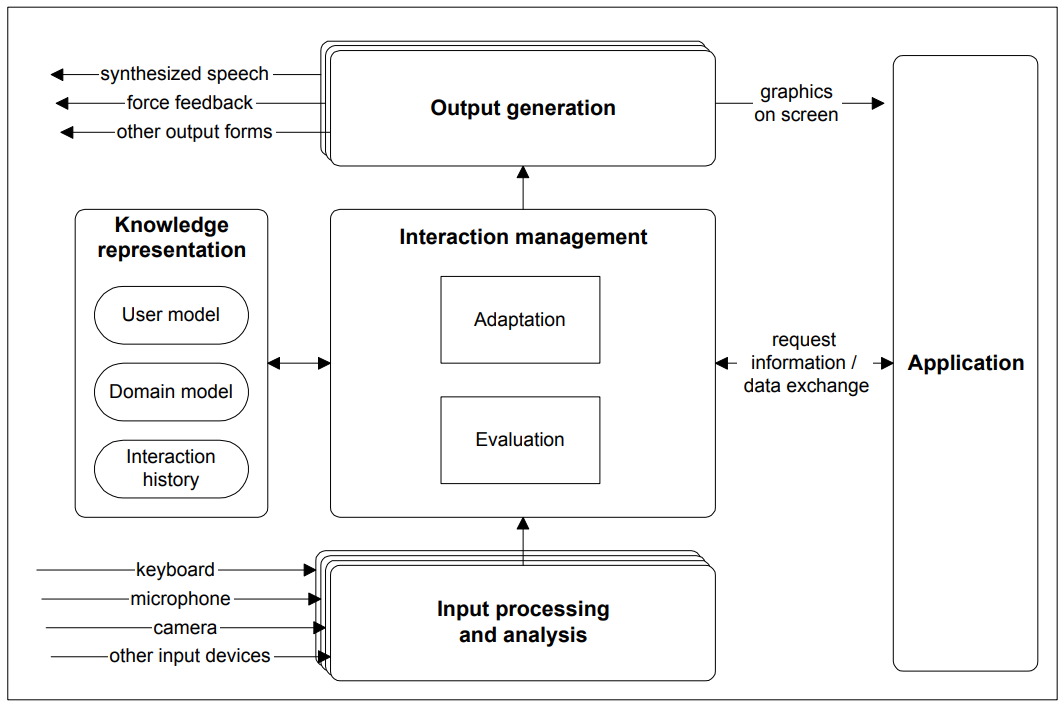
\includegraphics[scale=0.5]{images/iui_arch.png}}
\scnaddlevel{1}
    \scnrelfrom{источник}{Ehlert.P.IntellUserInterfIAS-2003art}
\scnaddlevel{-1}}

\scnhaselement{интеллектуальные технологии ввода}
\scnhaselement{моделирование пользователя}
\scnhaselement{модель пользователя}
\scnhaselement{адаптация к пользователю}
\scnhaselement{генерация пояснений}

\scnheader{моделирование пользователя}
\scnexplanation{Моделирование пользоваетля охватывает методы, которые позволяют системе поддерживать или делать выводы о пользователе на основе полученного ввода}
\lscnsource{Quote2.Ehlert.P.IntellUserInterfIAS-2003art.p4}

\scnheader{генерация пояснений}
\scnexplanation{Генерация пояснений охватывает все методы, которые позволяют системе объяснять свои результаты пользователю, например, речевой вывод, агенты интеллектуального интерфейса, тактильную обратную связь в среде виртуальной реальности.}
\lscnsource{Quote4.Ehlert.P.IntellUserInterfIAS-2003art.p4}

\scnheader{модель пользователя}
\scnexplanation{Для достижения персонализации IUI часто включают представление пользователя. Эти пользовательские модели регистрируют данные о поведении, знаниях и способностях пользователя. Новые знания о пользователе могут быть получены на основе истории ввода и взаимодействия пользователя с системой.}
\lscnsource{Quote5.Ehlert.P.IntellUserInterfIAS-2003art.p4}

\scnheader{адаптация к пользователю}
\scnexplanation{Адаптация к пользователю включает в себя все методы, которые позволяют адаптировать общение между человеком и машиной к разным пользователям и разным ситуациям, например, машинное обучение или понимание контекста.}
\lscnsource{Quote3.Ehlert.P.IntellUserInterfIAS-2003art.p4}

\scnheader{интеллектуальные технологии ввода}
\scnexplanation{Интеллектуальная технология ввода использует инновационные методы для получения ввода от пользователя. Эти методы включают в себя естественный язык, отслеживание и распознавание жестов, выражение лица распознавание и отслеживание взгляда среди прочего;}
\lscnsource{Quote1.Ehlert.P.IntellUserInterfIAS-2003art.p4}
\scnsuperset{речевой ввод}
\scnsuperset{естественно-языковой ввод}
\scnsuperset{жестовый ввод}
\scnsuperset{мимический ввод}

\scnheader{мимический ввод}
\scnsuperset{распознование лиц}
\scnaddlevel{1}
    \scnsuperset{распознование выражений лиц}
    \scnsuperset{отслеживание взгляда}
    \scnsuperset{чтение по губам}
\scnaddlevel{-1}

\scnheader{отслеживание взгляда}
\scnexplanation{Люди используют свои глаза с очень небольшим сознательным усилием. Большую часть времени мы автоматически смотрим на объект, над которым работаем. Чтобы четко видеть объект, необходимо переместить глаза так, чтобы объект оказался в центральной ямке, небольшой области в центре сетчатки. Ямка покрывает примерно один градус зрительной дуги. Из-за этого положение глаз человека обеспечивает довольно хорошую индикацию (с точностью до одного градуса ширины центральной ямки) точки фокусировки внимания человека на дисплее.}
\lscnsource{Quote3.Ehlert.P.IntellUserInterfIAS-2003.p18}

\scnheader{чтение по губам}
\scnexplanation{Проблема с распознаванием речи на основе акустического сигнала заключается в том, что оно очень плохо работает при большом количестве шума. Причина этого в том, что очень трудно отличить голос говорящего от других звуков. Идея чтения по губам заключается в том, что компьютер пытается определить, что кто-то говорит, просто глядя на движения губ человека, как глухой человек. Анализируя видеоизображения рта и используя геометрические признаки, такие как ширина и высота губ, можно определить наиболее вероятный звук (фонему).}
\lscnsource{Quote1.Ehlert.P.IntellUserInterfIAS-2003.p19}

\scnheader{жестовый ввод}
\scnexplanation{Люди часто используют жесты во время разговора, часто подсознательно. Наиболее часто используемые жесты связаны с речью, например, указывая на объект, о котором идет речь. Этот вид жестикуляции называется жестикуляцией. Жесты, функционирующие независимо от речи, называются автономными жестами, например язык жестов.}
\lscnsource{Quote1.Ehlert.P.IntellUserInterfIAS-2003art.p17}
\scnrelfrom{ввод}{жест}

\scnheader{жест}
\scnrelfromset{декомпозиция}{
    символический жест;
    дейктический жест;
    знаковый жест;
    пантомимический жест
}

\scnheader{символический жест}
\scnexplanation{Символические жесты имеют (единственное) вербальное и часто культурно-зависимое значение, например, знак «ОК» или язык жестов для глухих.}
\lscnsource{Quote2.Ehlert.P.IntellUserInterfIAS-2003.p17}

\scnheader{дейктический жест}
\scnexplanation{Дейктические жесты делаются путем указания или движения, чтобы привлечь внимание к какому-либо объекту или событию.}
\lscnsource{Quote3.Ehlert.P.IntellUserInterfIAS-2003.p17}

\scnheader{знаковый жест}
\scnexplanation{Знаковые жесты — это жесты, которые отображают информацию о размере, форме или ориентации объектов, пространственных отношениях и действиях, например, использование рук для обозначения размера пойманной рыбы).}
\lscnsource{Quote1.Ehlert.P.IntellUserInterfIAS-2003.p18}

\scnheader{пантомимический жест}
\scnexplanation{Пантомимические жесты состоят из манипулирования невидимым воображаемым объектом или инструментом, например, сжатие кулака и движение, обозначающее молоток).}
\lscnsource{Quote2.Ehlert.P.IntellUserInterfIAS-2003.p18}

\scnheader{естественно-языковой ввод}
\scnidtf{естественно-языковая система}
\scnrelfromset{декомпозиция}{
    распознавание речи;
    понимание языка;
    управление диалогом;
    запрос к базе данных;
    генерация ответа;
    речевой вывод
}

\scnheader{распознование речи}
\scnexplanation{Распознавание речи; преобразование входного речевого высказывания в строку из слов.}
\lscnsource{Quote1.Ehlert.P.IntellUserInterfIAS-2003art.p13}

\scnheader{понимание языка}
\scnexplanation{Понимание языка; анализ строки слов (насколько это возможно) для извлечения смыслового представления распознанного высказывания.}
\lscnsource{Quote2.Ehlert.P.IntellUserInterfIAS-2003art.p13}

\scnheader{управление диалогом}
\scnexplanation{Управление диалогом; управление взаимодействием или диалогом между системой и пользователем, что включает в себя координацию других компонентов системы.}
\lscnsource{Quote3.Ehlert.P.IntellUserInterfIAS-2003art.p13}

\scnheader{запрос к базе данных}
\scnexplanation{Запрос к базе данных; получение информации, запрошенной пользователем.}
\lscnsource{Quote4.Ehlert.P.IntellUserInterfIAS-2003art.p13}

\scnheader{генерация ответа}
\scnexplanation{Генерация ответа; спецификация текста, который должен быть выходным сообщением системы.}
\lscnsource{Quote5.Ehlert.P.IntellUserInterfIAS-2003art.p13}

\scnheader{речевой вывод}
\scnexplanation{Речевой вывод; фактическая генерация выходного сообщения с использованием синтеза речи или предварительно записанных фраз.}
\lscnsource{Quote6.Ehlert.P.IntellUserInterfIAS-2003art.p13}

\scnheader{мультимодальный интерфейс}
\scnexplanation{Идея мультимодальных интерфейсов заключается в использовании нескольких входных каналов при взаимодействии человека с компьютером. Вместо того, чтобы вводить только речь или текст, система может использовать распознавание изображений, чтобы смотреть на лицо или жесты пользователя. Таким образом, информация из одного режима взаимодействия может дополнять информацию, полученную из другого режима. Мультимодальные интерфейсы пытаются интегрировать речь, письменный текст, язык тела, жесты, движения глаз или губ и другие формы общения, чтобы лучше понимать пользователя и общаться более эффективно. Конечно, выбор используемых модальностей в мультимодальных интерфейсах во многом зависит от применения системы. Когда пользователи могут выбирать из нескольких способов взаимодействия с системой, система может стать доступной для более широкого круга пользователей, например для людей с ограниченными возможностями. Кроме того, мультимодальные пользовательские интерфейсы гораздо более надежны, чем обычные интерфейсы, по крайней мере, в теории. Обработка входных данных из одной модальности может быть упрощена за счет использования информации из другой, и пользователь может выбрать модальность, которая наименее подвержена ошибкам с учетом обстоятельств.}
\lscnsource{Quote1.Ehlert.P.IntellUserInterfIAS-2003art.p20}
\scnsuperset{слияние информации}

\scnheader{слияние информации}
\scnexplanation{Основным узким местом мультимодальных интерфейсов является объединение информации, полученной от используемых модальностей, в режиме реального времени. Все мультимодальные интерфейсы нуждаются в той или иной форме координации ввода или системы слияния для синхронизации связанного ввода.}
\lscnsource{Quote2.Ehlert.P.IntellUserInterfIAS-2003art.p20}
\scnrelfromset{декомпозиция}{
    слияние на уровне особенностей\\
    \scnaddlevel{1}
        \scnexplanation{Слияние на уровне функций уместно при объединении двух связанных модальностей, таких как обработка речи и движения губ. Преимуществом слияния на уровне функций является улучшенная скорость распознавания благодаря взаимодополняемости обоих входных каналов (взаимное устранение неоднозначности). Недостаток такой тесной интеграции обработки ввода заключается в том, что система должна переобучаться при изменении одной из модальностей ввода. Кроме того, обучение системы с несколькими модальностями с одновременным вводом данных намного сложнее, чем обучение одной модальности за раз.}
        \lscnsource{Quote3.Ehlert.P.IntellUserInterfIAS-2003art.p20}
    \scnaddlevel{-1};
    слияние на уровне семантики\\
    \scnaddlevel{1}
        \scnexplanation{Слияние на семантическом уровне намного проще. У него нет преимущества прямой дополнительной информации, но систему слияния на семантическом уровне гораздо проще создавать и расширять. Например, система может использовать несколько готовых методов распознавания, а новые модальности могут быть легко добавлены позже. Интеграция на семантическом уровне обычно выполняется либо путем объединения существующих данных, либо путем поиска отсутствующих данных. Последняя называется интеграцией на основе фреймов, когда системы пытаются заполнить недостающие слоты данных.}
        \lscnsource{Quote1.Ehlert.P.IntellUserInterfIAS-2003art.p20-21}
    \scnaddlevel{-1}
}

~\\
\scnauthorcomment{/* Далее идёт описание ранее неописанных компонентов интерфейса. */}
\scnheader{компонент ввода данных} 

...

    \scnsuperset{поле автозаполнения}
    \scnaddlevel{1}
        \scnidtf{autosuggest-field}
    \scnaddlevel{-1}
    
    \scnsuperset{строка навигатора}
    \scnaddlevel{1}
        \scnidtf{breadcrumb-bar}
        \scnidtf{панель навигации}
    \scnaddlevel{-1}
    
    \scnsuperset{управляющий элемент выбора даты в календаре}
    \scnaddlevel{1}
        \scnidtf{calendar-date-field}
    \scnaddlevel{-1}
    
    \scnsuperset{средство выбора цвета}
    \scnaddlevel{1}
        \scnidtf{color-palette}
        \scnidtf{палитра}
    \scnaddlevel{-1}
    
    \scnsuperset{поле со списком}
    \scnaddlevel{1}
        \scnidtf{list-field}
    \scnaddlevel{-1}
    
    \scnsuperset{ссылки на содержимое в текстовых элементах управления}
    \scnaddlevel{1}
        \scnidtf{content-link}
    \scnaddlevel{-1}
    
    \scnsuperset{управляющий элемент выбора даты}
    \scnaddlevel{1}
        \scnidtf{date-choice}
    \scnaddlevel{-1}
    
     \scnsuperset{форма}
     \scnaddlevel{1}
        \scnidtf{form}
     \scnaddlevel{-1}
     
     \scnsuperset{элемент управления рукописным вводом}
     \scnaddlevel{1}
        \scnidtf{handwriting-element}
     \scnaddlevel{-1}

\scnheader{поле автозаполнения}
\scnexplanation{Используйте AutoSuggestBox, чтобы предоставить список предложений, из которых пользователь по мере ввода текста может выбрать нужное.}
\scnaddlevel{1}
    \scneq{Quote1.Microsoft.WindowsDA-2011el}
\scnaddlevel{-1}

\scnheader{строка навигатора}
\scndefinition{Панель навигации предоставляет прямой путь к страницам или папкам в текущее расположение. Он часто используется для ситуаций, когда путь навигации пользователя (в файловой системе или системе меню) должен быть постоянно видимым, и пользователю может потребоваться вернуться к предыдущему расположению.}
\scnaddlevel{1}
    \scneq{Quote2.Microsoft.WindowsDA-2011el}
\scnaddlevel{-1}

\scnheader{управляющий элемент выбора даты в календаре}
\scndefinition{Управляющий элемент выбора даты в календаре — это раскрывающийся элемент управления, оптимизированный для выбора отдельной даты в представлении календаря, когда важна контекстная информация, например день недели или заполненность календаря. Вы можете изменить календарь таким образом, чтобы обеспечить дополнительный контекст или ограничить доступные даты.}
\scnaddlevel{1}
    \scneq{Quote3.Microsoft.WindowsDA-2011el}
\scnaddlevel{-1}

\scnheader{средство выбора цвета}
\scndefinition{Палитра используется для просмотра и выбора цвета. По умолчанию он позволяет пользователю перемещаться по цветам в цветовом спектре или указывать цвет в текстовых полях.}
\scnaddlevel{1}
    \scneq{Quote5.Microsoft.WindowsDA-2011el}
\scnaddlevel{-1}

\scnheader{поле со списком}
\scndefinition{Поле со списком (также известное как раскрывающийся список) позволяет представить список элементов, из которых пользователь может выбирать. Сначала поле со списком представлено в компактном состоянии, а затем развертывается для отображения списка элементов, доступных для выбора.}
\scnaddlevel{1}
    \scneq{Quote6.Microsoft.WindowsDA-2011el}
\scnaddlevel{-1}

\scnheader{ссылки на содержимое в текстовых элементах управления}
\scndefinition{Ссылки на содержимое позволяют вставлять в текстовые элементы управления форматированные данные. Благодаря этому пользователь может находить и использовать больше информации о людях и местах, не покидая вашего приложения.}
\scnaddlevel{1}
    \scneq{Quote10.Microsoft.WindowsDA-2011el}
\scnaddlevel{-1}

\scnheader{управляющий элемент выбора даты}
\scndefinition{Элемент выбора даты — это стандартизованный способ, позволяющий пользователям выбирать локализованное значение даты с помощью сенсорного ввода, мыши или клавиатуры.}
\scnaddlevel{1}
    \scneq{Quote11.Microsoft.WindowsDA-2011el}
\scnaddlevel{-1}

\scnheader{форма}
\scndefinition{Форма — это группа элементов управления, которые собирают данные пользователей и отправляют их. Формы обычно используются для страниц параметров, опросов, создания учетных записей и многого другого.}
\scnaddlevel{1}
    \scneq{Quote15.Microsoft.WindowsDA-2011el}
\scnaddlevel{-1}

\scnheader{элемент управления рукописным вводом}
\scndefinition{Элемент управления рукописным вводом позволяет включить в приложении базовые функции рукописного ввода}
\scnaddlevel{1}
    \scneq{Quote17.Microsoft.WindowsDA-2011el}
\scnaddlevel{-1}

\scnheader{интерактивный компонент пользовательского интерфейса}

    \scnsuperset{контекстное меню}
    \scnaddlevel{1}
        \scnidtf{раскрывающееся меню}
        \scnidtf{context-menu}
    \scnaddlevel{-1}
    
    \scnsuperset{панель команд}
    \scnaddlevel{1}
        \scnidtf{command-panel}
    \scnaddlevel{-1}
    
    \scnsuperset{карточка контакта}
    \scnaddlevel{1}
        \scnidtf{contact-card}
    \scnaddlevel{-1}
    
    \scnsuperset{диалоговые элементы управления}
    \scnaddlevel{1}
        \scnidtf{dialogue-element}
    \scnaddlevel{-1}
    
    \scnsuperset{расширитель}
    \scnaddlevel{1}
        \scnidtf{expander}
    \scnaddlevel{-1}
    
    \scnsuperset{представление пролистывания}
    \scnaddlevel{1}
        \scnidtf{scroller}
    \scnaddlevel{-1}
    
    \scnsuperset{всплывающе элементы}
    \scnaddlevel{1}
        \scnidtf{pop-up}
    \scnaddlevel{-1}
    
    \scnsuperset{представления списка и сетки}
    \scnaddlevel{1}
        \scnidtf{grid}
    \scnaddlevel{-1}
    
    \scnsuperset{гиперссылка}
    \scnaddlevel{1}
        \scnidtf{hyperlink}
    \scnaddlevel{-1}
    
    \scnsuperset{отображение карт}
    \scnaddlevel{1}
        \scnidtf{map-element}
    \scnaddlevel{-1}


\scnheader{контекстное меню}
\scndefinition{Всплывающие элементы меню используются в сценариях меню и контекстного меню для отображения списка команд или параметров, запрашиваемых пользователем.}
\scnaddlevel{1}
    \scneq{Quote18.Microsoft.WindowsDA-2011el}
\scnaddlevel{-1}

\scnheader{панель команд}
\scndefinition{Панели команд предоставляют пользователям удобный доступ к самым распространенным задачам приложения. Панели команд могут предоставлять доступ к командам приложения или страниц, работая с любым шаблоном навигации.}
\scnaddlevel{1}
    \scneq{Quote7.Microsoft.WindowsDA-2011el}
\scnaddlevel{-1}

\scnheader{карточка контакта}
\scndefinition{Карта контакта отображает контактные данные, такие как имя, номер телефона и адрес контакта. Карточка контакта также позволяет пользователю редактировать контактные данные. Можно выбрать, какую карточку следует отобразить: компактную карточку контакта или полную карточку контакта, которая содержит дополнительные сведения.}
\scnaddlevel{1}
    \scneq{Quote8.Microsoft.WindowsDA-2011el}
\scnaddlevel{-1}

\scnheader{диаологовые элемента управления}
\scndefinition{Диалоговые элементы управления — это модальные наложения пользовательского интерфейса, которые предоставляют контекстную информацию о приложении. Они блокируют взаимодействие с окном приложения, пока пользователь явно их не закроет. Они часто требуют от пользователя совершения каких-либо действий.}
\scnaddlevel{1}
    \scneq{Quote9.Microsoft.WindowsDA-2011el}
\scnaddlevel{-1}

\scnheader{расширитель}
\scndefinition{Элемент управления "Расширитель" позволяет отображать или скрывать менее важное содержимое, связанное с частью основного содержимого, которое всегда отображается. Элементы, содержащиеся в заголовке , всегда видны. Пользователь может развернуть и свернуть область содержимого , в которой отображается дополнительное содержимое, взаимодействуя с заголовком. Когда область содержимого развернута, она отправляет другие элементы пользовательского интерфейса из пути; он не накладывает другой пользовательский интерфейс. Может увеличиваться вверх или вниз.}
\scnaddlevel{1}
    \scneq{Quote12.Microsoft.WindowsDA-2011el}
\scnaddlevel{-1}

\scnheader{представление пролистывания}
\scndefinition{Используйте представление пролистывания для просмотра изображений или других элементов в коллекции, например фотографий в альбоме или элементов на странице описания продукта.}
\scnaddlevel{1}
    \scneq{Quote13.Microsoft.WindowsDA-2011el}
\scnaddlevel{-1}

\scnheader{всплывающий элемент}
\scndefinition{Всплывающий элемент — это контейнер с возможностью исчезновения, который отображает в качестве содержимого произвольный пользовательский интерфейс. Всплывающие элементы могут содержать другие вложенные всплывающие элементы или контекстные меню.}
\scnaddlevel{1}
    \scneq{Quote14.Microsoft.WindowsDA-2011el}
\scnaddlevel{-1}

\scnheader{гиперссылка}
\scndefinition{Гиперссылки используются для перехода в другую часть приложения, в другое приложение либо по указанному универсальному коду ресурса в отдельном приложении браузера.}
\scnaddlevel{1}
    \scneq{Quote16.Microsoft.WindowsDA-2011el}
\scnaddlevel{-1}

\scnheader{отображение карт}
\scndefinition{Карту можно показывать во всплывающем окне, называемом карточкой места, или в полнофункциональном элементе управления с картой.}
\scnaddlevel{1}
    \scneq{Quote19.Microsoft.WindowsDA-2011el}
\scnaddlevel{-1}

\end{small}
\end{SCn}